\documentclass[journal]{IEEEtran}
%DIF LATEXDIFF DIFFERENCE FILE
%DIF DEL report_1.tex     Wed Sep 21 08:20:15 2022
%DIF ADD report_1R1.tex   Wed Sep 21 08:38:25 2022

%DIF 3c3
%DIF < \usepackage{cite}
%DIF -------
\usepackage{natbib} %DIF > 
%DIF -------
\usepackage{orcidlink}
\usepackage{graphicx}  
%Please change to your image storage
\graphicspath{{../../Images/JPG/}}
\DeclareGraphicsExtensions{.pdf,.jpeg,.png}



\hyphenation{op-tical net-works semi-conduc-tor}
%DIF PREAMBLE EXTENSION ADDED BY LATEXDIFF
%DIF UNDERLINE PREAMBLE %DIF PREAMBLE
\RequirePackage[normalem]{ulem} %DIF PREAMBLE
\RequirePackage{color}\definecolor{RED}{rgb}{1,0,0}\definecolor{BLUE}{rgb}{0,0,1} %DIF PREAMBLE
\providecommand{\DIFadd}[1]{{\protect\color{blue}\uwave{#1}}} %DIF PREAMBLE
\providecommand{\DIFdel}[1]{{\protect\color{red}\sout{#1}}}                      %DIF PREAMBLE
%DIF SAFE PREAMBLE %DIF PREAMBLE
\providecommand{\DIFaddbegin}{} %DIF PREAMBLE
\providecommand{\DIFaddend}{} %DIF PREAMBLE
\providecommand{\DIFdelbegin}{} %DIF PREAMBLE
\providecommand{\DIFdelend}{} %DIF PREAMBLE
\providecommand{\DIFmodbegin}{} %DIF PREAMBLE
\providecommand{\DIFmodend}{} %DIF PREAMBLE
%DIF FLOATSAFE PREAMBLE %DIF PREAMBLE
\providecommand{\DIFaddFL}[1]{\DIFadd{#1}} %DIF PREAMBLE
\providecommand{\DIFdelFL}[1]{\DIFdel{#1}} %DIF PREAMBLE
\providecommand{\DIFaddbeginFL}{} %DIF PREAMBLE
\providecommand{\DIFaddendFL}{} %DIF PREAMBLE
\providecommand{\DIFdelbeginFL}{} %DIF PREAMBLE
\providecommand{\DIFdelendFL}{} %DIF PREAMBLE
\newcommand{\DIFscaledelfig}{0.5}
%DIF HIGHLIGHTGRAPHICS PREAMBLE %DIF PREAMBLE
\RequirePackage{settobox} %DIF PREAMBLE
\RequirePackage{letltxmacro} %DIF PREAMBLE
\newsavebox{\DIFdelgraphicsbox} %DIF PREAMBLE
\newlength{\DIFdelgraphicswidth} %DIF PREAMBLE
\newlength{\DIFdelgraphicsheight} %DIF PREAMBLE
% store original definition of \includegraphics %DIF PREAMBLE
\LetLtxMacro{\DIFOincludegraphics}{\includegraphics} %DIF PREAMBLE
\newcommand{\DIFaddincludegraphics}[2][]{{\color{blue}\fbox{\DIFOincludegraphics[#1]{#2}}}} %DIF PREAMBLE
\newcommand{\DIFdelincludegraphics}[2][]{% %DIF PREAMBLE
\sbox{\DIFdelgraphicsbox}{\DIFOincludegraphics[#1]{#2}}% %DIF PREAMBLE
\settoboxwidth{\DIFdelgraphicswidth}{\DIFdelgraphicsbox} %DIF PREAMBLE
\settoboxtotalheight{\DIFdelgraphicsheight}{\DIFdelgraphicsbox} %DIF PREAMBLE
\scalebox{\DIFscaledelfig}{% %DIF PREAMBLE
\parbox[b]{\DIFdelgraphicswidth}{\usebox{\DIFdelgraphicsbox}\\[-\baselineskip] \rule{\DIFdelgraphicswidth}{0em}}\llap{\resizebox{\DIFdelgraphicswidth}{\DIFdelgraphicsheight}{% %DIF PREAMBLE
\setlength{\unitlength}{\DIFdelgraphicswidth}% %DIF PREAMBLE
\begin{picture}(1,1)% %DIF PREAMBLE
\thicklines\linethickness{2pt} %DIF PREAMBLE
{\color[rgb]{1,0,0}\put(0,0){\framebox(1,1){}}}% %DIF PREAMBLE
{\color[rgb]{1,0,0}\put(0,0){\line( 1,1){1}}}% %DIF PREAMBLE
{\color[rgb]{1,0,0}\put(0,1){\line(1,-1){1}}}% %DIF PREAMBLE
\end{picture}% %DIF PREAMBLE
}\hspace*{3pt}}} %DIF PREAMBLE
} %DIF PREAMBLE
\LetLtxMacro{\DIFOaddbegin}{\DIFaddbegin} %DIF PREAMBLE
\LetLtxMacro{\DIFOaddend}{\DIFaddend} %DIF PREAMBLE
\LetLtxMacro{\DIFOdelbegin}{\DIFdelbegin} %DIF PREAMBLE
\LetLtxMacro{\DIFOdelend}{\DIFdelend} %DIF PREAMBLE
\DeclareRobustCommand{\DIFaddbegin}{\DIFOaddbegin \let\includegraphics\DIFaddincludegraphics} %DIF PREAMBLE
\DeclareRobustCommand{\DIFaddend}{\DIFOaddend \let\includegraphics\DIFOincludegraphics} %DIF PREAMBLE
\DeclareRobustCommand{\DIFdelbegin}{\DIFOdelbegin \let\includegraphics\DIFdelincludegraphics} %DIF PREAMBLE
\DeclareRobustCommand{\DIFdelend}{\DIFOaddend \let\includegraphics\DIFOincludegraphics} %DIF PREAMBLE
\LetLtxMacro{\DIFOaddbeginFL}{\DIFaddbeginFL} %DIF PREAMBLE
\LetLtxMacro{\DIFOaddendFL}{\DIFaddendFL} %DIF PREAMBLE
\LetLtxMacro{\DIFOdelbeginFL}{\DIFdelbeginFL} %DIF PREAMBLE
\LetLtxMacro{\DIFOdelendFL}{\DIFdelendFL} %DIF PREAMBLE
\DeclareRobustCommand{\DIFaddbeginFL}{\DIFOaddbeginFL \let\includegraphics\DIFaddincludegraphics} %DIF PREAMBLE
\DeclareRobustCommand{\DIFaddendFL}{\DIFOaddendFL \let\includegraphics\DIFOincludegraphics} %DIF PREAMBLE
\DeclareRobustCommand{\DIFdelbeginFL}{\DIFOdelbeginFL \let\includegraphics\DIFdelincludegraphics} %DIF PREAMBLE
\DeclareRobustCommand{\DIFdelendFL}{\DIFOaddendFL \let\includegraphics\DIFOincludegraphics} %DIF PREAMBLE
%DIF COLORLISTINGS PREAMBLE %DIF PREAMBLE
\RequirePackage{listings} %DIF PREAMBLE
\RequirePackage{color} %DIF PREAMBLE
\lstdefinelanguage{DIFcode}{ %DIF PREAMBLE
%DIF DIFCODE_UNDERLINE %DIF PREAMBLE
  moredelim=[il][\color{red}\sout]{\%DIF\ <\ }, %DIF PREAMBLE
  moredelim=[il][\color{blue}\uwave]{\%DIF\ >\ } %DIF PREAMBLE
} %DIF PREAMBLE
\lstdefinestyle{DIFverbatimstyle}{ %DIF PREAMBLE
	language=DIFcode, %DIF PREAMBLE
	basicstyle=\ttfamily, %DIF PREAMBLE
	columns=fullflexible, %DIF PREAMBLE
	keepspaces=true %DIF PREAMBLE
} %DIF PREAMBLE
\lstnewenvironment{DIFverbatim}{\lstset{style=DIFverbatimstyle}}{} %DIF PREAMBLE
\lstnewenvironment{DIFverbatim*}{\lstset{style=DIFverbatimstyle,showspaces=true}}{} %DIF PREAMBLE
%DIF END PREAMBLE EXTENSION ADDED BY LATEXDIFF

\begin{document}

\title{A Brief Group Introduction}


\author{Qingyu~Luo\orcidlink{0000-0001-6263-2917}, ~\IEEEmembership{Postgraduate,~XDU,}
        Junxiao~Li\orcidlink{0000-0003-0133-5307},~\IEEEmembership{Postgraduate,~XDU,}
        Jiawen~Wang\orcidlink{0000-0003-3636-7405},~\IEEEmembership{Postgraduate,~XDU,}
        and~Chaozhuo~Hua\orcidlink{0000-0002-5126-3818},~\IEEEmembership{Postgraduate,~XDU}% <-this % stops a space
}


% The paper headers
\markboth{Journal of \LaTeX\ Class Files,~Vol.~14, No.~8, August~2015}%
{Shell \MakeLowercase{\textit{et al.}}: Bare Demo of IEEEtran.cls for IEEE Journals}




% make the title area
\maketitle

% As a general rule, do not put math, special symbols or citations
% in the abstract or keywords.
\begin{abstract}
	This article is a simple introduction to the group members, which includes the photos, personality, group responsibility, and research interests of the group members. Through the reference of the document, and on the basis of the IEEE official template, we have completed this article.
\end{abstract}

% Note that keywords are not normally used for peerreview papers.
\begin{IEEEkeywords}
IEEE, Git Repository, Member Introduction
\end{IEEEkeywords}




\IEEEpeerreviewmaketitle



\section{Introduction}

\IEEEPARstart{A} clear and simple Recommended Structure of a repository for scientific Projects is crucial for the entire scientific research project.So we build our own git repository based on \DIFdelbegin \DIFdel{Recommend Structure of A Repository proposed by Professor Frery~\mbox{%DIFAUXCMD
\cite{2020A}}\hskip0pt%DIFAUXCMD
}\DIFdelend \DIFaddbegin \DIFadd{the recommend structure proposed by \mbox{%DIFAUXCMD
\citet{2020A}}\hskip0pt%DIFAUXCMD
}\DIFaddend .
At the same time, a clear understanding of the internal characteristics of each team member is also helpful for follow-up study and research. 
Based on this, we submitted a document written \DIFdelbegin \DIFdel{by }\DIFdelend \DIFaddbegin \DIFadd{in }\DIFaddend \LaTeX\DIFdelbegin \DIFdel{\ in the warehouse}\DIFdelend , which contains a detailed introduction of each team member.


\section{\DIFdelbegin \DIFdel{team member}\DIFdelend \DIFaddbegin \DIFadd{Team Members}\DIFaddend }

Qingyu Luo is a person who is keen to explore how technology can improve people's production and life, and has the qualities of diligence and innovation. He is reliable and inspiring in teamwork.

Junxiao Li has enthusiasm, is a man of focus, isn't afraid of dealing with difficulties, and would like \DIFdelbegin \DIFdel{tofigure }\DIFdelend \DIFaddbegin \DIFadd{to figure }\DIFaddend out which troubles with him. %DIF > %% ACF Strange closing; please be clear about this.
Have working experience in student clubs, \DIFdelbegin \DIFdel{with }\DIFdelend \DIFaddbegin \DIFadd{he has }\DIFaddend a strong sense of responsibility and work coordination ability. 
\DIFdelbegin \DIFdel{Have }\DIFdelend \DIFaddbegin \DIFadd{He has }\DIFaddend experience in mathematical modeling competitions and a certain foundation of programming modeling.

Jiawen Wang is a cheerful, honest and upright girl from Xi'an, an ancient capital city. With the experience of participating in mathematical modeling competitions, she has some programming modeling \DIFdelbegin \DIFdel{foundation }\DIFdelend \DIFaddbegin \DIFadd{background }\DIFaddend and hopes to go far in the academic path.

Chaozhuo Hua, an intelligent young man, lively and lovely is his indispensable feature, who has a strong heart, also, \DIFdelbegin \DIFdel{Optimistic }\DIFdelend \DIFaddbegin \DIFadd{optimistic }\DIFaddend and persistent personality, aggressive, dare to face difficulties and challenges.

\DIFdelbegin %DIFDELCMD < \bibliographystyle{unsrt}
%DIFDELCMD < %%%
%DIF < change it into your path
\DIFdelend \DIFaddbegin \bibliographystyle{IEEEtranN}
\small
\DIFaddend \bibliography{../Common/reference}


\begin{IEEEbiography}[{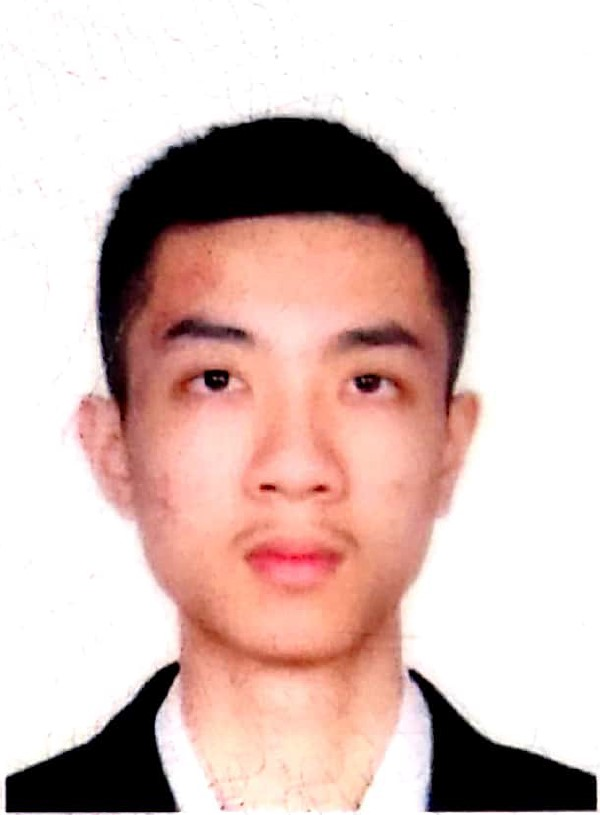
\includegraphics[width=1in,height=1.25in,clip,keepaspectratio]{Qingyu.jpg}}]{Qingyu Luo}
(Postgraduate,~XDU) Received the B.E. degree in Microelectronics from the Xidian University, Xi'an, in 2018. His main research direction is model pruning.

\end{IEEEbiography}


 \begin{IEEEbiography}[{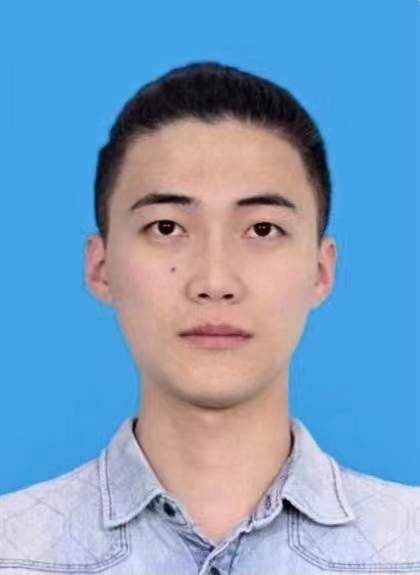
\includegraphics[width=1in,height=1.25in,clip,keepaspectratio]{Junxiao.jpg}}]{Junxiao Li}
(Postgraduate,~XDU) Received the
C.S. degree in C.S. from the Xi'dian University, Xi'an, in 2017, and won 2020
American College Students mathematical Modeling
Competition Meritorious. Her main research direction is satellite image 3D construction.
\end{IEEEbiography}

  \begin{IEEEbiography}[{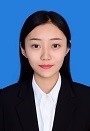
\includegraphics[width=1in,height=1.25in,clip,keepaspectratio]{Jiawen.jpg}}]{Jiawen Wang}
    studying in the School of Artificial Intelligence at Xi'an University of Electronic Science and Technology, and her main research interests are remote sensing image processing and analysis.
 \end{IEEEbiography}

 \begin{IEEEbiography}[{\includegraphics[width=1in,height=1.25in,clip,keepaspectratio]{Chaozhuo.jpg}}]{Chaozhuo Hua}
(Postgraduate,~XDU)Received a bachelor's degree in Artifificial Intelligence from the Xidian University in 2018, main research in 
Remote sensing image target detection.
\end{IEEEbiography}


\end{document}


